% !TeX spellcheck = en_US
% !TeX encoding = UTF-8
\chapter{Theoretical foundation}

\section{Stress Definition and Measurement}
Stress, a term frequently used in everyday language aswell as in scientific domain, is an individual's response to situations perceived as challenging, threatening, or overwhelming. Stress is an unpleasant emotional state that individuals experience when confronted with demands that they perceive as taxing or exceeding their coping capabilities \parencite{stress2}.

Stress, also called the "fight-or-flight" response, is an evolutionary adaptation that equips someone to respond to demanding situations rapidly. When faced with a potential threat or challenge, the human body instinctively readies itself for self-defence or swift evasion. The body's sympathetic nervous system is responsible for this response, which rapidly increases the production of stress hormones like cortisol, adrenaline, and noradrenaline \parencite{1}.

The hormonal changes cause a range of bodily reactions, including acceleration of the heartbeat, muscle tension, changes in posture, increased blood pressure, rapid breathing, and heightened sensory alertness etc. One can objectively measure these bodily changes, which generally fall into two categories: physical and physiological changes.

Physical measures focus on observable bodily changes that occur under stress. These include alterations in facial expressions, variations in the rate of eye blinking and pupil dilation, changes in body posture and movement patterns. These visible markers offer insights into an individual's stress levels.

Physiological measures, in contrast, involve using sensors to detect internal bodily changes indicative of stress. A range of biomarkers is employed for this purpose, including \gls{HRV}  and \gls{HR}, \gls{GSR} electrodermal activity, respiratory patterns and cortisol levels. These biomarkers provide a more direct and quantifiable insight into the body's response to stress, making them valuable tools in stress assessment.

Experts specializing in research also meticulously design standardized questionnaires for the subjective evaluation of stress, which has been a longstanding approach to understanding individual stress levels. These questionnaires are structured to accurately capture an individual's perceived stress levels and their reactions to various stressors. This subjective methods are crucial as they offer insights into the personal experiences and perceptions of stress, which may not always be evident through objective measures.

\section{Subjective Measures \gls{gptmo}}

Subjective ratings, such as self-report questionnaires, have
been commonly used as a direct method to estimate levels of mental stress in humans in an experimental setting.
\parencite{aigram}. Participants are asked to answer a variety of
questions about their experiences in the experiment. There have been a different variety of questionnaires and tests used to investigate the emotional state or perceived stress from the human participants in experimental setting. Some of the most widely used ones are \gls{SAM} \parencite{SAM}, \gls{NASA-TLX} \parencite{tlx}, \gls{PSS} \parencite{pss} etc.

 The \gls{SAM} is a non-verbal pictorial assessment technique designed to measure emotional response and affective reaction to diverse stimuli \parencite{SAM}. Administered typically at the conclusion of each experimental task, it asks participants to assess their emotions and affective state on a scale from 1 to 9 across three dimensions: valence (the nature of the emotion, ranging from positive like relaxation to negative such as fear), arousal (the intensity of the emotion), and dominance (the extent to which the emotion is perceived as controllable).


 \GLS{NASA-TLX} is extensively used in various research studies to evaluate mental stress levels. Notably, \textcite{tlxstress} implemented this tool to assess the mental workload of surgeons during endoscopy training. In a similar vein, \textcite{Zaki} applied NASA-TLX within the context of smart factories to scrutinize factors like task complexity, time pressure, and collaboration duration, all contributing to mental stress.

 Primarily, NASA-TLX aims to measure perceived workload across different tasks, particularly in high-stress environments. It seeks to capture a comprehensive picture of stress and workload through subjective user experiences. The tool does this by evaluating six key dimensions: Mental Demand, Physical Demand, Temporal Demand, Performance, Effort, and Frustration, each playing a role in the overall task load assessment for an individual. The evaluation process incorporates a NASA-developed technique for gauging the relative significance of these factors in the experienced workload. For each of the six dimensions, NASA-TLX employs a 21-point bipolar scale, allowing participants to range their workload assessment between two extremes, such as "Low/High." Furthermore, the process involves presenting pairs of rating scale labels, prompting subjects to choose which label is more pertinent to their cognitive workload experience in the task. This selection pattern enables the assignment of a weight to each cognitive load factor, culminating in an overall score that aligns with a specific subject's experience.

 \textcite{tlxstress} demonstrates the use of the NASA-TLX for assessing mental stress by interpreting workload measurements as indicators of stress levels. This approach highlights NASA-TLX's utility in evaluating how task demands can translate into mental stress.
 
 In our research, NASA-TLX emerged as the most fitting tool for assessing stress in the context of the external stimuli of human-robot collaborative tasks. Stress, as a multifaceted experience, varies subjectively in perception. It might arise in response to workload (our focus area) but also encompasses factors such as emotional responses, individual coping mechanisms, and various personal and environmental influences. Characterized often by feelings of strain, anxiety, or pressure, stress responds to both internal and external stimuli. Given our specific objective to assess stress related to the external stimuli of the task, other questionnaires like the Perceived Stress Scale (PSS), Trier Inventory for the Assessment of Chronic Stress (TICS) \parencite{tics} - which measures general chronic stress over a period, or the Daily Stress Inventory (DSI) \parencite{dsi} - evaluating daily stress events, did not align with our requirements.

While subjective questionnaire is a powerful tool to measure stress levels directly, it is important to mention their limitations. The reliance on self-reporting means it's subject to individual biases and may not accurately reflect real-time stress levels. People might not always be able to accurately introspect and report their feelings or may inadvertently skew their responses based on what they think researchers want to hear.




\section{Objective Measures \gls{gptmo}}
Objective measures of stress include measuring of physiological and physical measures by means of sensors. These sensors are either placed on the human body to measure bodily changes in an unobtrusive manner or at a distance in case of physical measurements. Objective measures of stress are free from human intervention and hence cannot be biased. 
The two sensors we used to collect biosignals objectively are the Empatica E4 and the OptiTrack Motion Capture System. They are introduced below:

\subsection{Empatica E4}
The Empatica E4 \parencite{empatica} (see \autoref*{fig:empatica}) wristband is a versatile and compact device designed to capture a wide range of physiological data in real time. 
It has four sensors: a \gls{PPG} sensor, which measures \gls{BVP}; an \gls{EDA} sensor, which is used for measuring \gls{GSR}; a 3-axis Accelerometer to capture motion-based activity and an infrared thermopile to reads skin temperature (ST) \parencite{empa}. Its unobtrusive nature makes it comfortable to wear, while its comprehensive data collection capabilities have made it an invaluable asset.

The Empatica E4 wristband collects \gls{BVP} data using the \gls{PPG} with a process that involves emitting green and red light from LEDs into the skin and measuring the reflected light with a sensor(see \autoref{fig:ppg}). The green light, absorbed by the blood, provides a pulsatile signal corresponding to the cardiovascular pulse wave used to determine heartbeats. The red light acts as a reference to correct for motion artifacts. Algorithms then process this data within the wristband to output the \gls{BVP}, from which the interbeat interval (IBI)—the time between heartbeats—is calculated, offering a non-invasive method to monitor heart rate continuously.\parencite{emp2}

\gls{EDA} is measured by detecting the electrical conductance across the skin, which is an indirect indicator of the sweat gland activity influenced by the sympathetic nervous system. To obtain these measurements, Empatica employs a method that relies on passing a minimal electrical current between two electrodes that are in contact with the skin, typically placed on the bottom wrist.

The wristband also includes a 3-axis accelerometer and an infrared thermopile, which can track body temperature and movement, providing a comprehensive overview of the wearer's physiological state.



\begin{figure}[!htbp]
	\centering
	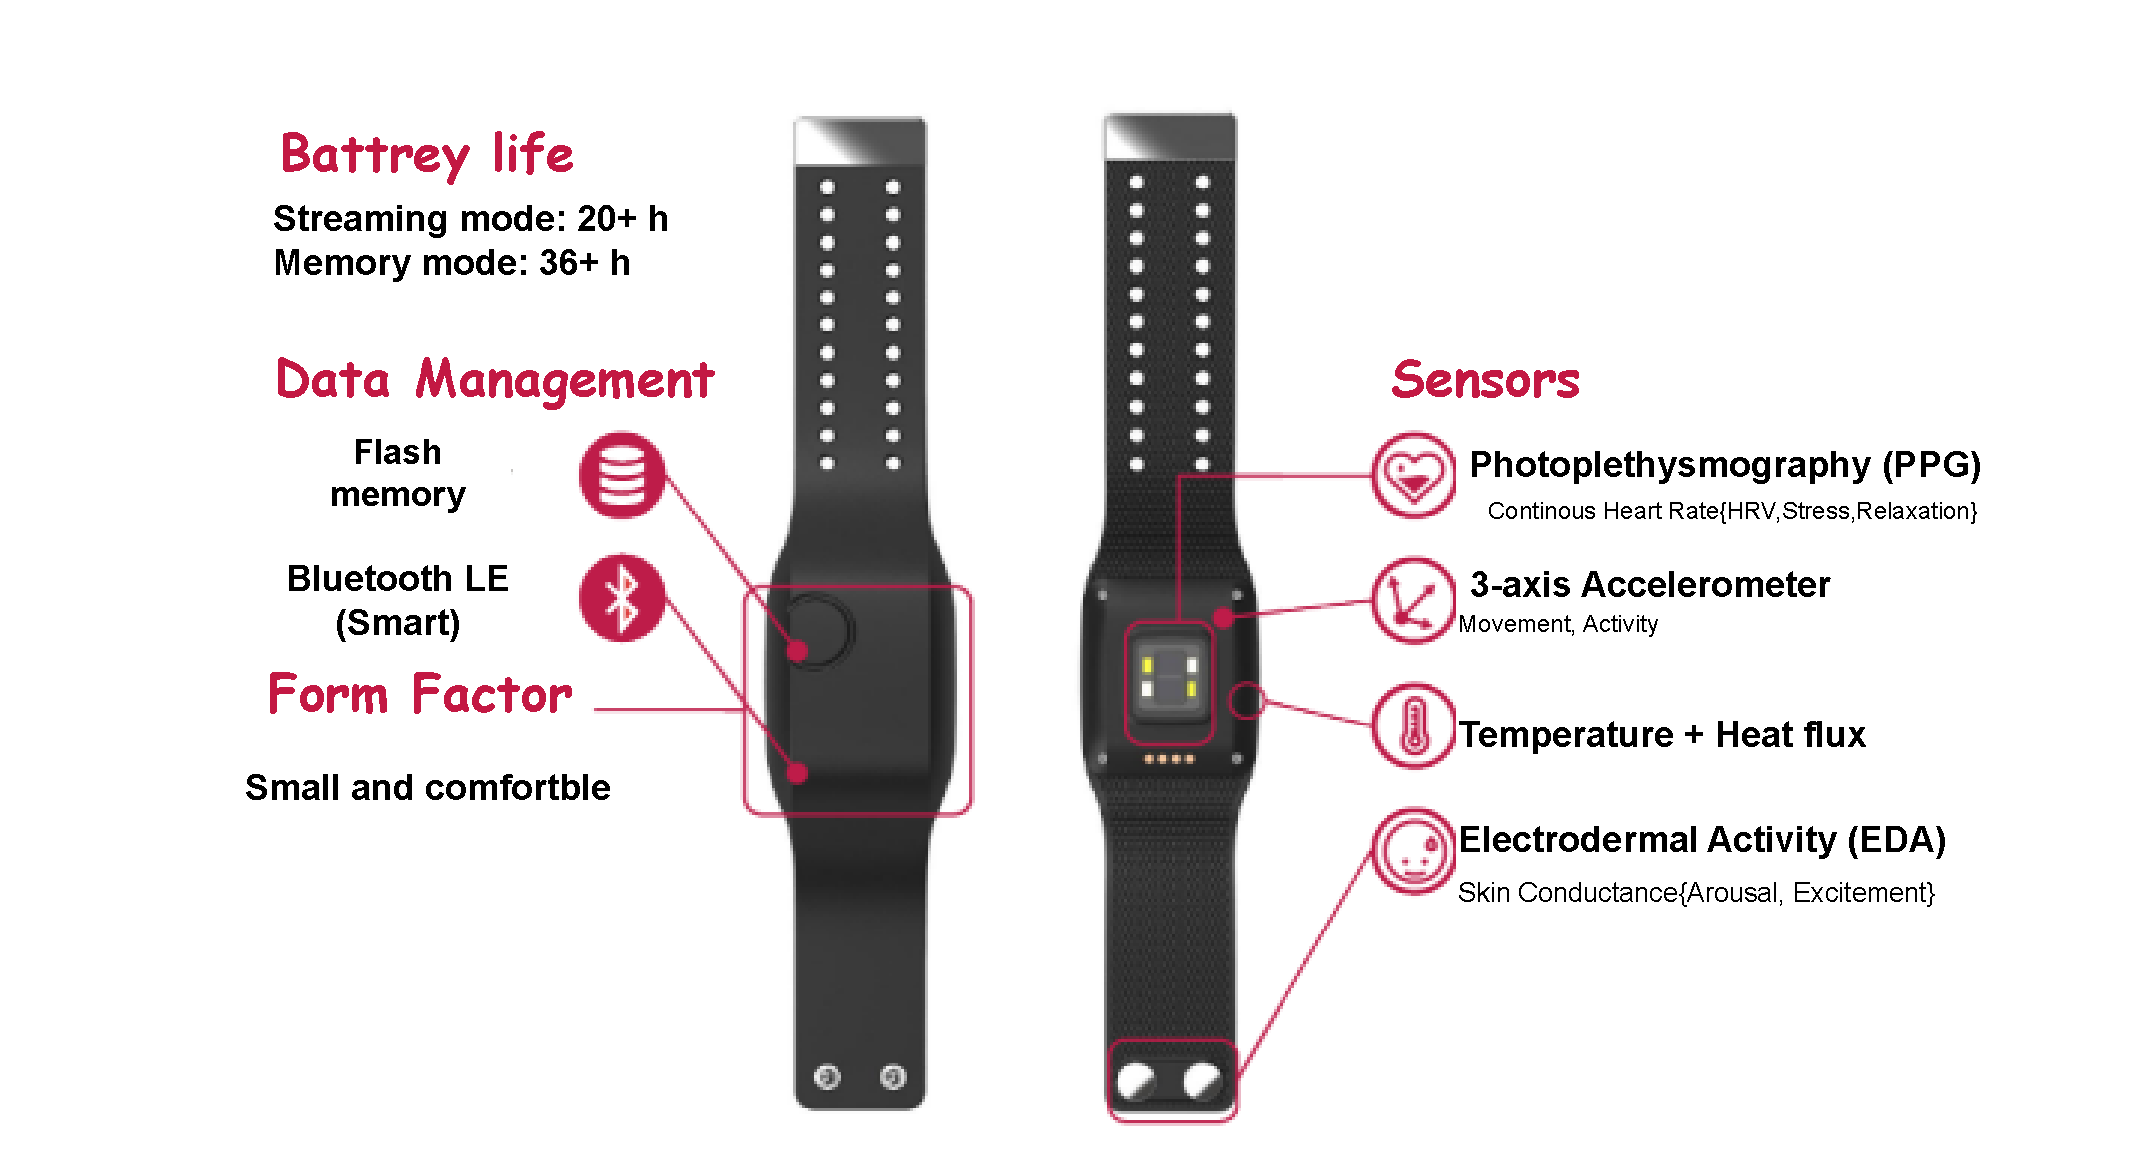
\includegraphics[width=0.8\columnwidth]{images/e4.drawio.pdf}
	\caption{Empatica E4 features \parencite{emp}}
	\label{fig:empatica}
\end{figure}


\subsection*{Photoplethysmogram-PPG }
\label{subsec:PPGtheory}

Photoplethysmogram (PPG) also known as  Blood Volume Pulse (BVP) are non-invasive optical techniques used to monitor changes in blood volume. They rely on the principles of light absorption and reflection to capture valuable information about cardiovascular activity. \gls{PPG} sensors commonly found in wearable devices obtain \GLS{BVP} signals by transmitting light into the skin and measuring the amount of light either transmitted through or reflected back.\parencite{ppg} 

When the heart beats, it propels blood through the circulatory system, causing periodic changes in the volume of blood vessels. PPG sensors emit light into the tissue and measure the amount of light that is either absorbed or reflected back. During each heartbeat, blood absorbs more light, leading to a decrease in the amount of light detected by the sensor. Between heartbeats, when blood flow is less pulsatile, more light is detected.\parencite{ppg2}

The resulting waveforms from PPG typically consist of a series of peaks and troughs, with each peak corresponding to a heartbeat (systole) and each trough representing the resting period between beats (diastole). By analyzing the time intervals between these peaks, the heart rate can be calculated. This heart rate measurement is fundamental and provides valuable information about a person's cardiovascular health and overall fitness level. It serves as a key metric in various applications, including exercise tracking, medical diagnosis and in our case here stress assessment.

Furthermore, PPG signals enable the assessment of HR and \gls{HRV}. HRV is the variation in time between successive heartbeats and is an essential indicator of the autonomic nervous system's activity. By analyzing the subtle changes in the intervals between PPG peaks, HRV can be quantified. High HRV typically indicates a healthy heart and a well-balanced autonomic nervous system, while reduced HRV can be associated with stress, illness, or various medical conditions. HRV analysis provides insights into the body's ability to adapt to different situations and is valuable for assessing stress levels, mental well-being, and overall cardiovascular health.

Other measures that can be derived from PPG data include  and estimation of blood oxygen saturation levels (SpO2), valuable for respiratory and circulatory health assessment. PPG can also be used to estimate respiration rate, reveal vasomotor activity changes associated with the autonomic nervous system, emotions, or vascular health, and provide insights into arterial stiffness and blood flow dynamics as well as blood pressure. First derivative and second derivates of PPG signals can also be analyzed. The first derivative (Velocity Plethysmogram, VPG) and the second derivative (Acceleration Plethysmogram, APG) features can be used for  blood pressure estimation etc.\parencite{apg}


\begin{figure}[!htbp]
    \centering
    % First image
    \begin{subfigure}[b]{0.55\columnwidth}
        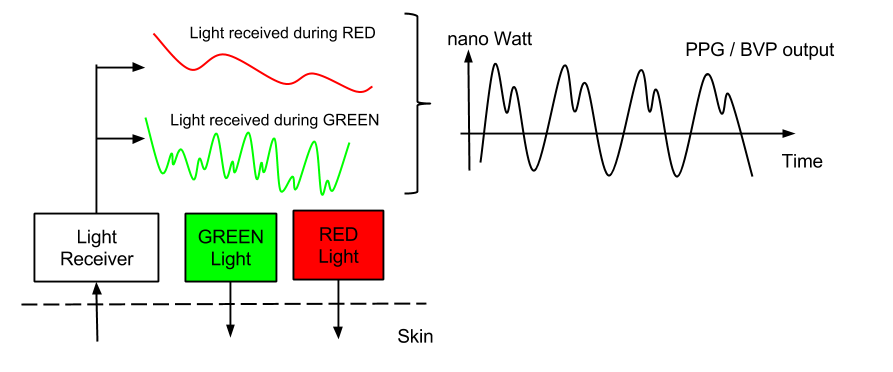
\includegraphics[width=\textwidth]{images/PPG.png}
        \caption{PPG process}
        \label{fig:ppg}
    \end{subfigure}
    % Second image
    \begin{subfigure}[b]{0.35\columnwidth}
        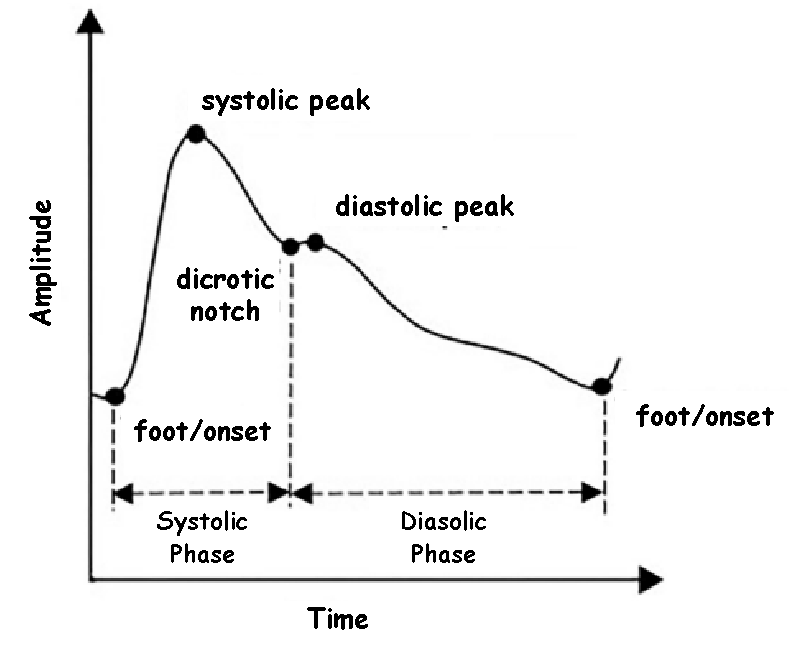
\includegraphics[width=\textwidth]{images/ppg2.pdf}
        \caption{Typical PPG Waveform}
        \label{fig:phone2}
    \end{subfigure}
    \caption{\parencite{emp} \parencite{apg}}
    \label{fig:phone}
\end{figure}



\subsection*{Electrodermal Activity-EDA \gls{gptmo}}
\label{subsec:EDAtheory}

Electrodermal Activity (EDA), also known as the galvanic skin response(GSR), is a way to measure changes in how our skin conducts electricity. Even moderate amounts of sweating that are not observable at the skin surface can alter skin electrical conductivity. The more the body sweats, the more conductive the skin becomes, and this change can be measured to infer physiological or psychological states.More specifically  EDA measures the skin's electrical conductance changes, which depend on the quantity of sweat secreted by eccrine sweat glands in the hypodermis of the palmar and plantar regions. Sweat secreted in the palmar and plantar regions is caused mainly by central nervous activity related to affective and cognitive states, including mental or emotional sweating \parencite{eda23}. Thus, EDA becomes one of the promising noninvasive methods widely used in detecting stress and emotion. EDA is a powerful method for real-time measurement and could be used as an index of emotional or cognitive stimulation related to stress.\parencite{gellman2020behavioral}.EDA is useful in several ways: it shows how we respond emotionally, helps us see how our body reacts to stress etc. It acts as a biomarker for emotional responsiveness and serves as a key indicator for stress-related bodily responses. 

Electrodermal Activity (EDA) comprises two main components: the tonic and phasic components. The tonic component, also known as skin conductance level (SCL), reflects slow and consistent changes in the signal's background. In contrast, the phasic components, referred to as skin conductance response (SCR) or spontaneous fluctuation of skin response, are the rapid and momentary fluctuations within the signal that occur within specific time intervals \parencite*{hernando2017feature}. SCR appears in response to stimuli activating the sympathetic nervous system. Consequently, SCR can be linked to a stimulus and can be valuable in measuring cognitive stress levels. However, directly extracting the components of EDA isn't straightforward.

When EDA sensors measure skin conductivity (SC) signals, they typically yield results in microsiemens. To extract the SCL and SCR components accurately, it is necessary to deconvolve the SC signals \parencite[postnote]{alexander2005separating}. Without proper separation of the original SC signals, overlapping SCRs can lead to less precise information during feature extraction . Therefore, it is crucial to perform deconvolution to distinguish the SCR and SCL signals effectively.

\begin{figure}[!htbp]
	\centering
	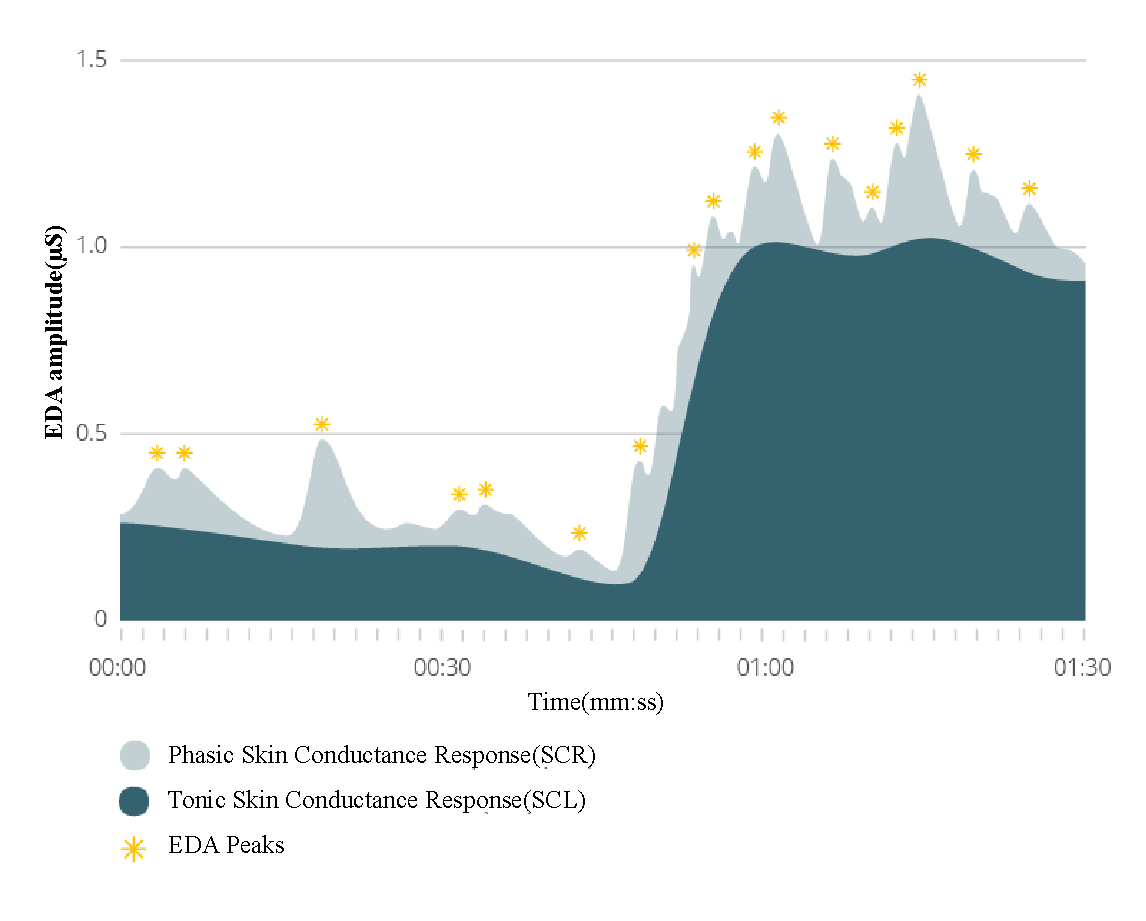
\includegraphics[width=0.8\columnwidth]{images/eda.pdf}
	\caption{EDA Example signal - \parencite{eda}}
	\label{fig:eda sig}
\end{figure}

\subsection*{Skin Temperature }
Other Physiological signal measured by the Empatica E4 is the skin temperature. Typically, the normal range for skin temperature lies between 33.5 and 36.9°C but changes in skin temperature can be connected to the stressful and anxious conditions \parencite{emp2}
Skin temperature is strongly correlated to the heart activity and sweat reaction of an individual, so when a person is sweating, their skin temperature increases thus being a measure of increased stress levels.


\subsection{Motion Capture}
\label{subsec:mocap}
The OptiTrack Motion Capture System is a motion capture system that uses an array of 12 high-speed cameras equipped with advanced optics and infrared sensors. These cameras are positioned to cover a designated area, creating a three-dimensional space where every movement is tracked and recorded. The system detects reflective markers placed on key points of a subject's body. As the subject moves within the camera's field of view, the system tracks the spatial position and orientation of these markers, seamlessly translating physical movements into digital data. 

For tracking the human body, the system uses a set of 25 marker points, which are placed at strategic points as shown in {\autoref{fig:opti3}}. This configuration ensures a thorough capture of the upper body movements. The calibration process is a critical step where each marker on the subject's body is meticulously mapped onto a digital skeleton model. This mapping ensures that the system can accurately track the movements of each marker in relation to the body's overall structure.The system individually tracks each marker as the subject moves, allowing for a detailed representation of motion.
The Motive software, integral to the OptiTrack system, plays a key role here. It enables users not only to visualize the movements in real time but also to record and analyze the data. The software translates the positional data of the markers into a skeletal animation, offering a clear and dynamic representation of the subject's movements.

\begin{figure}[!htbp]
    \centering
    % First image
    \begin{subfigure}[b]{0.45\columnwidth}
        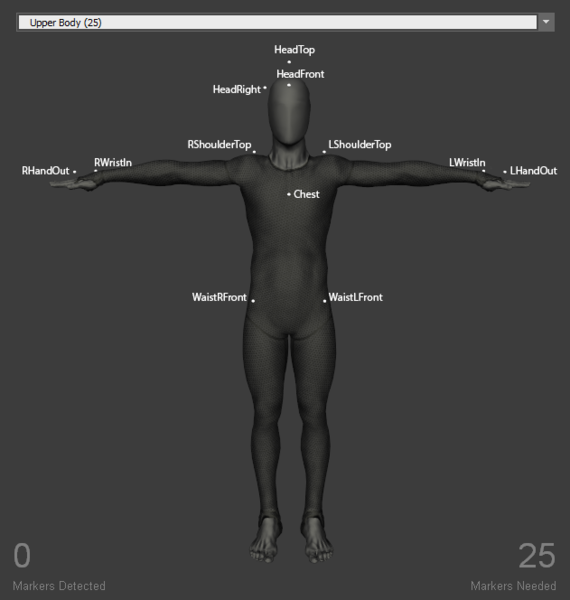
\includegraphics[width=\textwidth]{images/skleton.png}
        \caption{Front View }
        \label{fig:opti1}
    \end{subfigure}
    % Second image
    \begin{subfigure}[b]{0.45\columnwidth}
        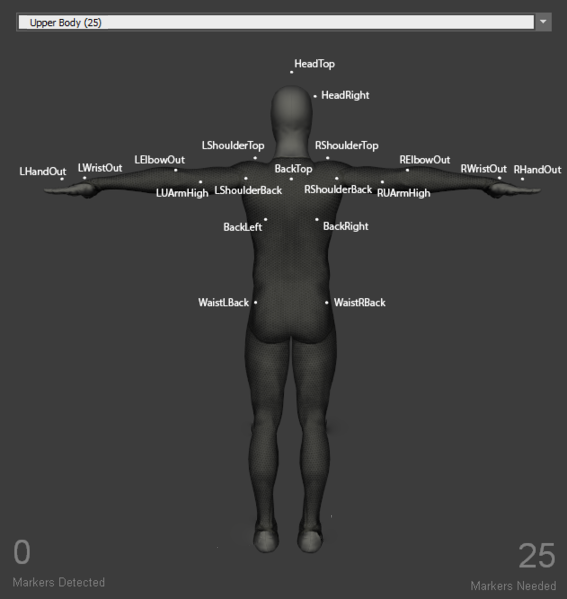
\includegraphics[width=\textwidth]{images/skeleton2.png}
        \caption{Back View }
        \label{fig:opti2}
    \end{subfigure}
    \caption{25 Upper Body Marker Set \parencite{opti}}
    \label{fig:opti3}
\end{figure}

\begin{comment}
\subsection*{Other Non-Wearable Sensors}
Other measures to help assess stress can be obtained by means of non-wearable sensors. These sensors are not directly connected to the body of the individual, but they measure stress either using physical measures, behavioral measures or computer vision based methods. Physical measures are one in which some observable parameters of the human body like human pupil dilation, human speech, human eye activity, and body postures are recorded, whereas, on the other hand, behavioral measures are the ones in which human stress is measured based on some behavioral changes such as face touching, biting of lips, tapping of legs etc. The third and last type of non-wearable sensors used for human stress measurement is computer vision-based sensors like a video camera and thermal imaging. \parencite{arsalan}.
These measures can give more information about the 
\end{comment}

\section{UR10 robot and Collision Avoidance \gls{gptmo}}
The UR10 is part of the Universal Robots family of \gls{Cobots}, designed to collaborate directly with humans in a shared workspace. This robotic arm with six joints is highly flexible, has a reach of 1300 mm, and can handle a payload of up to 10 kg, making it suitable for a wide range of applications and collaborative tasks.\autoref{fig:ur10} shows the ur10 with its 6 rotatory joints.

Despite its capability to perform complex tasks, the UR10 does not inherently possess collision avoidance strategies. Its default response to encountering a collision is typically to halt operations to prevent any damage or injury, relying on built-in safety features that comply with industrial safety standards. However, innovative research and development have sought to enhance the UR10's capabilities with advanced collision avoidance strategies.

%\paragraph{Human Body Representation}
It is necessary to simplify the human body tracked using the motion capture system in \autoref{label:subsec:mocap}  for ease of computation in collision avoidance trajectory planning. The simplified human body is modelled using line swept spheres \parencite{larsen}. A swept sphere, also known as a capsule, is the volume of a sphere that is swept along a straight line. It resembles a cylinder in shape, but it is simpler for distance metric computational purposes. 

\begin{figure}[!htbp]
    \centering
    % First image
    \begin{minipage}[b]{0.40\columnwidth}
        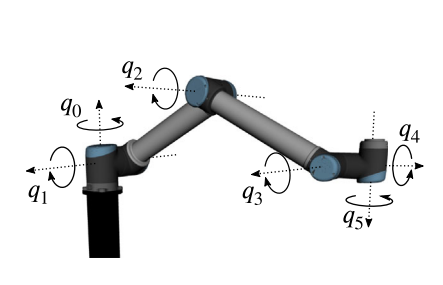
\includegraphics[width=\textwidth]{images/ur10.png}
        \caption{6 DOF UR10 taken from \parencite{max}}
        \label{fig:ur10}
    \end{minipage}
    % Second image
    \begin{minipage}[b]{0.40\columnwidth}
        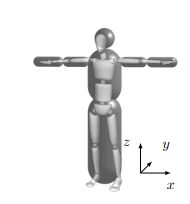
\includegraphics[width=\textwidth]{images/reduced body.png}
        \caption{Simplified human model taken from \parencite{renz1}} 
        \label{fig:reduced}
    \end{minipage}
\end{figure}

Seven spherical volumes make up the human body model: a sphere represents the head, while these swept sphere volumes represent the rest of the body parts, such as the arms, the torso and the parts below the hip is depicted by these swept spheres. This method effectively and precisely captures the human form and its movements in a simplistic manner, reducing complexity and increasing computational speeds. 
\autoref{fig:reduced} shows the simplfied human body model superimposed on the skeleton model of the motion capture system.
The motion capture system continuously monitors and records the individual's movements. This information is then fed into the robot's planning system, allowing it to maneuver and modify its actions adeptly in response to the human's changing position and movements.

%\paragraph{Collision Avoidance Strategies}
This thesis discusses three different levels of collision strategies.

\begin{figure}[!htbp]
	\centering
	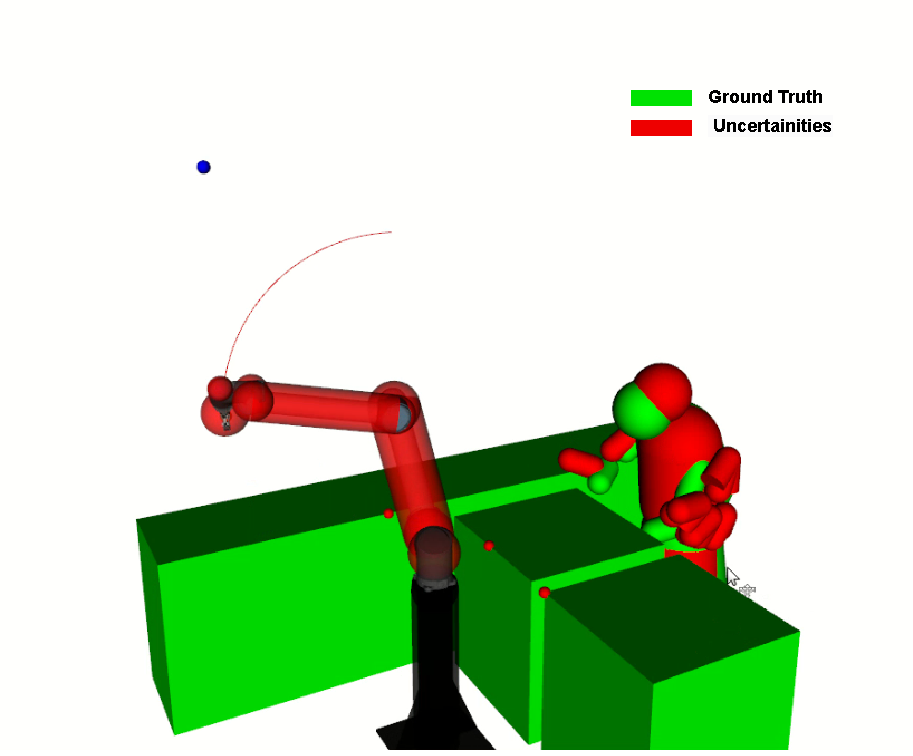
\includegraphics[width=0.8\columnwidth]{images/uncertainities (1).pdf}
	\caption{Predictive Collision Avoidance}
	\label{fig:pred}
\end{figure}

The first one already discussed is the default collision strategy of the UR10 robot, where it stops at a collision.

The second one uses dynamic collision avoidance, which tracks moving humans and tries to avoid them in real-time. It focuses \gls{MPC}, a method that anticipates and adapts to changes in the environment, including moving obstacles.
This control scheme by \textcite{max} integrates online trajectory optimization with MPC. This approach enables the robot to adjust its movement in real-time, considering potential collisions and task variations. The prediction model within MPC approximates the robot's joint velocities and positions, facilitating efficient adaptation to dynamic obstacles.
The control system is structured in a cascaded manner. The outer loop handles MPC, planning optimal movement trajectories, while the inner loop consists of tracking controllers for velocity references. This architecture effectively decouples the complex dynamics of robot motion control, simplifying the computational process.\parencite{max}

The third predictive collision avoidance strategy is predicting the future human motion. One approach for predicting human motion is the extrapolation of the human skeleton's joint states in joint space using Polynomial Estimation (PE) methods as done by \textcite{renz1}. This technique involves fitting a polynomial to past joint angles in a least-squares sense and predicting future joint states, which includes the joint angles and their velocities and accelerations. These predictions inherently come with some degree of uncertainty, especially as the prediction horizon extends further into the future.
To represent this uncertainty, a \GLS{GMM} is applied, which describes multiple potential future extrapolations. Each extrapolation is defined by observations of the errors between the predicted joint states and the actual (ground truth) joint states at different time steps. These errors are time-dependent, with the assumption that errors increase for predictions further into the future.\parencite{renz2}.

The GMM consists of several components, each representing a normal distribution with its own mean and covariance matrix. These components collectively form a probabilistic model of the potential errors in joint state predictions over time. The parameters of the GMM are updated using an Expectation-Maximization (EM) algorithm, which maximizes the likelihood of the observed data (the past prediction errors). However, due to computational constraints, the GMM is not updated with every new extrapolation but rather at set intervals considering the most recent set of extrapolations.

This GMM approach allows for the estimation of uncertainties in a real-time capable manner, which is crucial for adjusting the robot's motion plan to avoid collisions with humans dynamically and safely.


\section{Stress Classification \gls{gptmg}}
The classification of stress levels in individuals has been the subject of extensive research, leading to the development of various methods. Stress classification is a supervised learning problem, a category of machine learning. In supervised learning, the model is trained on a labelled dataset, meaning each input data point is associated with a known output label. In the context of stress classification, these labels represent different stress states, such as 'stressed' or 'not stressed'. The model learns from this training data, enabling it to make predictions or classify new, unseen data based on recognised patterns.

Among the various techniques employed for stress classification, Support Vector Machines (SVM), K-nearest neighbors (KNN), Logistic Regression, and Decision Trees are notable for their widespread use. These methods each have unique foundational concepts and operational mechanisms:

\begin{itemize}
    \item \textbf{Support Vector Machines (SVM)}: SVMs are known for their efficacy in classifying non-linearly separable data. They function by identifying the optimal hyperplane that separates different classes in the feature space.
    \item \textbf{K-Nearest Neighbors (KNN)}: KNN classifies data based on the similarity principle, considering how closely a new data point resembles existing points in the training set. This method is particularly useful when dealing with irregular decision boundaries.
    \item \textbf{Logistic Regression}: Commonly used for binary classification, Logistic Regression computes the probability that a given input belongs to a particular class, ideal for cases where the output is a probability or a binary decision.
    \item \textbf{Decision Trees}: Decision Trees employ a tree-like model of decisions, where each node represents a feature, each branch represents a decision rule, and each leaf represents an outcome. They are simple to understand and interpret and are useful for both classification and regression tasks.
\end{itemize}

Research by \textcite{machine}, \textcite{1}, \textcite{review2021}, and \textcite{Sharma2012} has been instrumental in reviewing, summarizing, and comparing these commonly utilized methods in stress classification. Their analyses provide insights into the efficiency, applicability, and specificities of these classifiers, offering a deeper understanding of their role in stress level classification. This section aims to present an overview of the background information of these chosen classifiers.

\subsection*{Support Vector Machine}

Support Vector Machine (SVM) is a supervised machine learning algorithm widely used for classification and regression tasks. At its core, SVM aims to find the optimal hyperplane that separates data points of different classes in a high-dimensional space. This separation is achieved to maximise the margin between the data points of other classes, ensuring the best possible classification.


The process of selecting the best hyperplane for data separation follows a methodical approach, adaptable for both binary and multiclass scenarios. Here's a general overview of the steps involved:

% Drawing Lines with Kernel Functions
To separate data points into distinct classes, SVM employs kernel functions, which can be denoted as \( K(\mathbf{x}_i, \mathbf{x}_j) \). These kernel functions transform the input data into a higher-dimensional space where a hyperplane can be used for separation.

% Identifying Support Vectors
The support vectors are the data points closest to the hyperplane and satisfy the following conditions:
\begin{align}
    \mathbf{w} \cdot \mathbf{x}_+ + b &= +1, \quad \text{for positively labeled data,} \\
    \mathbf{w} \cdot \mathbf{x}_- + b &= -1, \quad \text{for negatively labeled data.}
\end{align}
These points are vectors \(\mathbf{x}_+\) and \(\mathbf{x}_-\) that lie on the boundary of the margin.

% Calculating the Margin
The margin is defined as the distance between the support vectors and the hyperplane. It can be calculated as:
\begin{equation}
    \text{margin} = \frac{2}{\|\mathbf{w}\|}.
\end{equation}

% Selecting the Optimal Hyperplane
The optimal hyperplane is the one that maximizes the margin. The objective function to maximize the margin while classifying the training data correctly is given by:
\begin{equation}
    \max_{\mathbf{w}, b} \frac{2}{\|\mathbf{w}\|}, \quad \text{s.t. } y_i(\mathbf{w} \cdot \mathbf{x}_i + b) \geq 1, \quad \forall i.
\end{equation}
This can also be equivalently written as a minimization problem:
\begin{equation}
    \min_{\mathbf{w}, b} \frac{1}{2} \|\mathbf{w}\|^2, \quad \text{s.t. } y_i(\mathbf{w} \cdot \mathbf{x}_i + b) \geq 1, \quad \forall i.
\end{equation}

By solving this optimization problem, SVM finds the optimal hyperplane that classifies the data with the maximum margin, enhancing the generalization ability of the classifier.


The SVM stands out from other classifiers that also use lines or hyperplanes due to its strategy of utilizing the maximum margin separating hyperplanes. By focusing on this maximum margin, the SVM enhances its ability to correctly predict the classification of new, previously unseen instances. The chosen hyperplane effectively determines how an unknown sample is classified, falling into one class or another based on which side of the hyperplane it lies. This approach ensures that the classifier is not only effective but also robust in its predictions, making SVM a valuable tool in a wide range of classification applications.

Support Vector Machines (SVMs) are particularly well-suited for the task of stress classification from physiological data. By constructing an optimal hyperplane in a high-dimensional feature space, SVMs can efficiently differentiate between stressed and non-stressed states based on various biosignals. The mathematical foundation of SVM in the context of stress classification can be represented as follows:

Below is the table of common kernel functions used in SVM:
\begin{table}[!ht]
    \centering
    \caption{Kernels}
    \label{tab:kernels}
    \begin{tabular}{|l|c|}
    \hline
    \textbf{Kernel}        & \textbf{Expression}                               \\ \hline
    Linear Kernel          & \( K(\mathbf{x}_i, \mathbf{x}_j) = \mathbf{x}_i^\top \mathbf{x}_j \)                \\ \hline
    Polynomial Kernel      & \( K(\mathbf{x}_i, \mathbf{x}_j) = (\mathbf{x}_i^\top \mathbf{x}_j + c)^d \)       \\ \hline
    Sigmoid Kernel         & \( K(\mathbf{x}_i, \mathbf{x}_j) = \tanh(\beta \mathbf{x}_i^\top \mathbf{x}_j + \theta) \) \\ \hline
    RBF                    & \( K(\mathbf{x}_i, \mathbf{x}_j) = \exp(-\gamma \|\mathbf{x}_i - \mathbf{x}_j \|^2) \)   \\ \hline
    \end{tabular}
    \end{table}
    
    \begin{figure}[!htbp]
        \centering
        % First image
        \begin{minipage}[b]{0.45\columnwidth}
            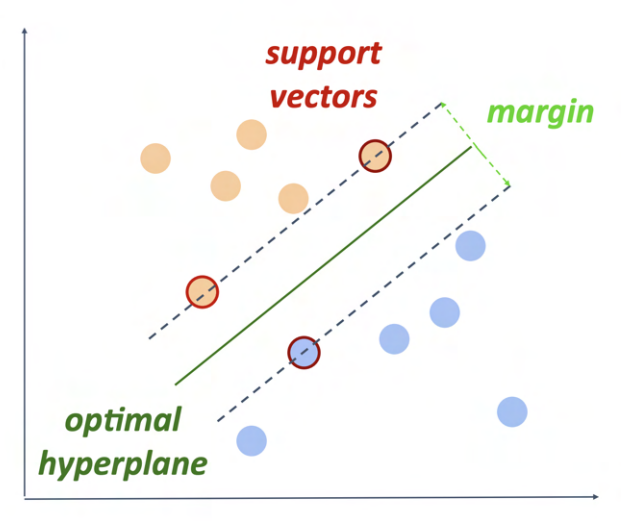
\includegraphics[width=\textwidth]{images/svm.png}
            \caption{SVM taken from \parencite{ml}}
            \label{fig:ur10}
        \end{minipage}
        % Second image
        \begin{minipage}[b]{0.45\columnwidth}
            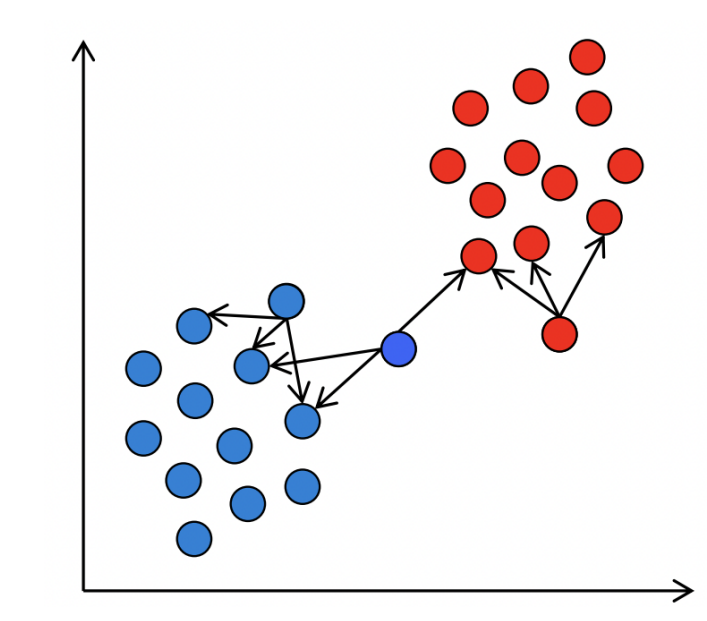
\includegraphics[width=\textwidth]{images/knn.png}
            \caption{kNN taken from \parencite{ml}} 
            \label{fig:reduced}
        \end{minipage}
    \end{figure}
    




    \subsection*{K-Nearest Neighbors (KNN)}
    K-Nearest Neighbors (KNN) is a versatile algorithm used in supervised machine learning, predominantly employed for classification and, to some extent, regression tasks. It operates on the principle of classifying new data points based on the majority class among its nearest neighbors in the feature space. The proximity of neighbors is determined using distance metrics, such as the Euclidean distance and Manhattan distance, calculated by the following formulas:

    \begin{equation}
        \text{Euclidean Distance}(\mathbf{x}_i, \mathbf{x}_j) = \sqrt{\sum_{k=1}^{n} (x_{ik} - x_{jk})^2}
    \end{equation}
    
    \begin{equation}
        \text{Manhattan Distance}(\mathbf{x}_i, \mathbf{x}_j) = \sum_{k=1}^{n} |x_{ik} - x_{jk}|
    \end{equation}
    
    The choice of `k', the number of nearest neighbors to consider, is critical. A smaller `k' can make the model sensitive to noise, while a larger `k' can lead to high computational costs and may include less relevant neighbors. Optimal `k' is often determined through cross-validation.
    
    Some variations of KNN employ weighted voting, where closer neighbors have more influence on the classification than more distant ones, enhancing the accuracy in certain scenarios.
    
    KNN is effective for stress classification in datasets where stress indicators form distinct clusters. In physiological data, for instance, patterns of stress responses might cluster, enabling KNN to differentiate between stressed and non-stressed states. While KNN's simplicity and effectiveness are advantageous for smaller datasets, it faces challenges like high computational cost in large datasets and sensitivity to irrelevant features. Feature selection and dimensionality reduction techniques are employed to mitigate these issues.
    
    In conclusion, KNN's approach of classifying data based on nearest neighbors, along with its adaptability to distance metrics like Euclidean and Manhattan distances, makes it a valuable tool for stress classification. Key considerations for its effective application include dataset size, feature relevance, and the optimal choice of `k'.
    
\subsection*{Logistic Regression}

Logistic Regression is a widely-used statistical method in supervised machine learning, particularly suited for binary classification tasks. It predicts the probability of a certain class or event based on one or more independent variables, making it ideal for outcomes that are categorical, such as 'yes/no', 'true/false', or 'stressed/not stressed'. The fundamental concept of Logistic Regression is to estimate the probabilities of different possible outcomes of a categorically distributed dependent variable, given a set of independent variables. This is achieved using the logistic function, an S-shaped curve that can map any real-valued number to a value between 0 and 1. The logistic function, also known as the sigmoid function, is central to Logistic Regression and is defined as:

\begin{equation}
    \text{Sigmoid}(\theta) = \frac{1}{1 + e^{-\theta}}
\end{equation}

Here, \( \theta \) represents the linear combination of the input features. The model expresses the probability that each input belongs to a certain class as a function of this logistic function. Logistic Regression is particularly effective for binary classification tasks, such as stress classification. It models the probability that a given input is 'stressed'. The model outputs a probability score, and a threshold, usually set at 0.5, is used to classify the input into one of two classes. 

While traditionally used for binary classification, Logistic Regression can be extended to multi-class classification problems, such as classifying inputs into three distinct classes. Techniques like One-vs-Rest (OvR) and Multinomial Logistic Regression allow for handling multiple classes. The Softmax function is often employed in these cases to generalize the Logistic Regression model for multiple classes.

Logistic Regression is valued for its simplicity and interpretability, requiring low computational resources. It assumes a linear relationship between the independent variables and the logit of the dependent variable, and may not perform well with complex relationships in data, where methods like SVM or Neural Networks could be more suitable. In conclusion, Logistic Regression's probabilistic outputs and straightforward implementation make it a popular choice for binary classification tasks, including stress level classification, and its adaptability to multi-class classification further enhances its utility in various applications.

   